\section{Direct Memory Access (DMA)}
There are 3 forms of I/O :
\begin{enumerate}
  \item Basic
  \item Interrupt-processed
  \item DMA
\end{enumerate}
\textbf{Direct Memory Access} (DMA): Provides direct access to memory while the microprocessor is temporarily disables.
\newline
\textbf{Applications}: DRAM refresh, video displays for refreshing the screen, disk memory system read/write etc.

\begin{figure}[h!]
  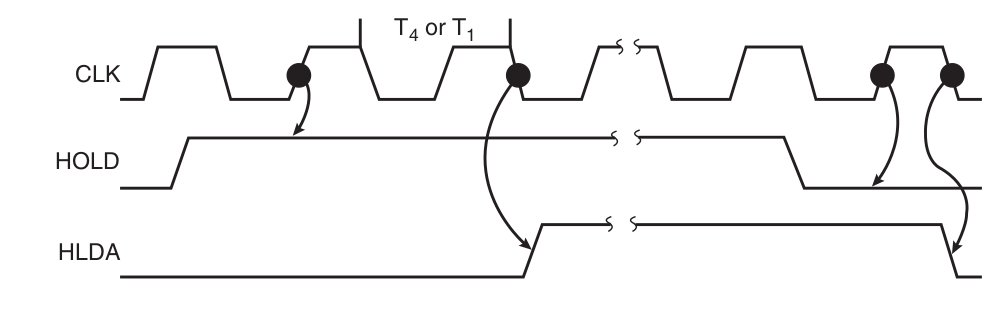
\includegraphics[width = 0.8\textwidth]{./figures/HOLD_HLDA.png}
  \caption{HOLD and HLDA timing for the microprocessor.}
\end{figure}

\begin{itemize}
  \item HOLD is sampled in the middle of any clock cycle. As soon as the microprocessor recognized the hold, it stops executing software and enters hold cycle.
  \item HOLD is a higher priority than INTR and NMI. Interrupts take effect at the end of an instruction, while a HOLD takes effect in the middle of an instruction.
  \item The only microprocessor pin having a higher priority than HOLD is RESET
  \item The HLDA becomes active to indicate that the microprocessor has places its buses at high-impedence state.
  \item \textbf{HOLD}: DMA requested
  \item \textbf{HLDA}: DMA grant output.
  \item \textbf{DMA read}: Transfers data from memory to I/O ($\overline{MRDC},~\overline{IOWC}$)
  \item \textbf{DMA write}: Transfers data from memory to I/O ($\overline{MWTC},~\overline{IORC}$)


\end{itemize}

\subsection{Control signal generation in 8086/8088}
\begin{figure}[h!]
  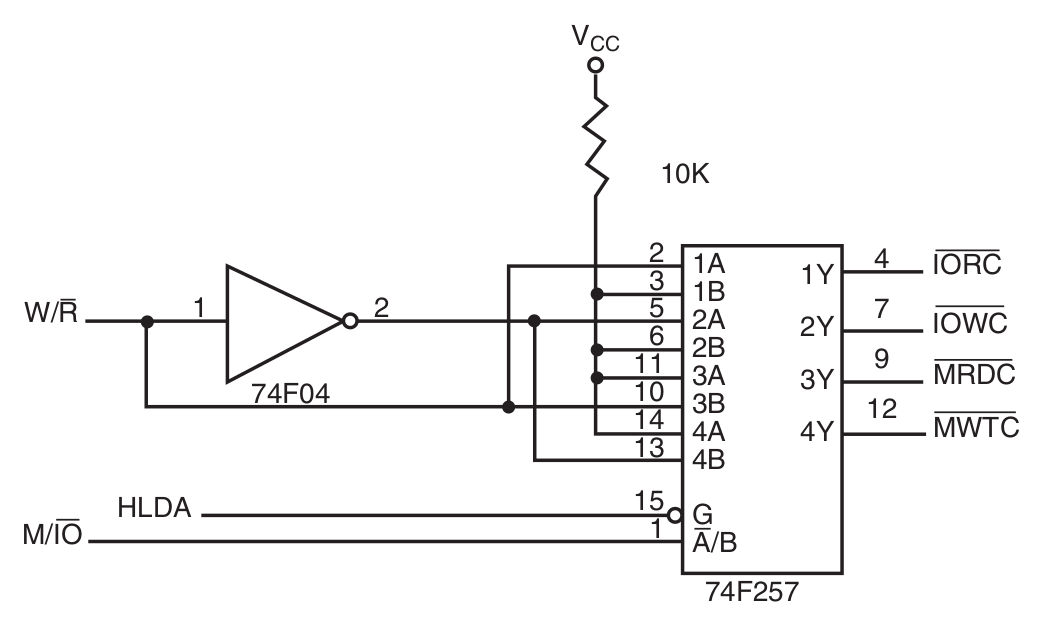
\includegraphics[width = 0.8\textwidth]{./figures/Control_Signal_Gen.png}
  \caption{A circuit that generates system control signals in a DMA environment.}
\end{figure}

\begin{table}[h!]
\centering
\begin{tabular}{ |p{1cm}|p{1cm}|p{1cm}|p{3cm}|  }
\hline
M/$\overline{IO} $ & W/$ \overline{R} $ & Output   \\
\hline
M               & W $\longrightarrow$ NOT & $\overline{MWTC}$ \\
M               & $\overline{R}$          & $\overline{MRDC}$ \\
$\overline{IO}$ & W $\longrightarrow$ NOT & $\overline{IOWC}$ \\
$\overline{IO}$ & $\overline{R}$          & $\overline{IORC}$ \\
\hline
\end{tabular}
\caption{Control signal generation in 8086/8088}
\label{table:15}
\end{table}

\subsection{8237 DMA Controller}
A special purpose microprocessor whose job is high-speed data transfer between memory and I/O. \newline
Pins of 8237 : \newline
\begin{description}
  \item[DREQ3 - DREQ0] DMA request input (four-channel)
  \item[DACK3 - DACK0] DMA channel acknowledge.
  \item[HRQ] HOLD request
  \item[HLDA] HOLD acknowledge

  \item[$\overline{EOP}$] End of Process; Used to terminate a DMA process or to signal the end of a DMA transfer.

  \item[$\overline{IOR}$] I/O read is a bidirectional pin used during programming and during a DMA write cycle.
  \item[$\overline{IOW}$] I/O write is a bidirectional pin used during programming and during a DMA read cycle.
  \item[$A_0 - A_3$] These address pins select an internal register during programming and also provide part of the DMA transfer address during a DMA action. The address pins are outputs that provide part of the DMA transfer address during a DMA action.
  \item[$DB_0 - DB_7$] The data bus pins are connected to the microprocessor data bus connec-
  tions and are used during the programming of the DMA controller.
  \item[CLK] The clock input is connected to the system clock signal as long as that
  signal is 5 MHz or less. In the 8086/8088 system, the clock must be
  inverted for the proper operation of the 8237.
  \item[$\overline{CS}$] Chip select enables the 8237 for programming. The CS pin is normally
  connected to the output of a decoder. The decoder does not use the
  8086/8088 control signal IO>M ( M>IO ) because it contains the new
  memory and I/O control signals ( MEMR , MEMW , IOR , and IOW ).
  \item[Internal Register] \textbf{************SELF-STUDY*********}

\end{description}

\subsection{Arithmetic Coprocessor}
8087, 80287, 80387X, ..... \newline
  \subsubsection{80x87}
  Ability to multiply, divide, add, Substract, Square Root, Partial tangent, Partial arctangent, tangent
  \textbf{Data types}: 16- , 32- , 64-bit signed integers; 18-digit BCD data, and 32- , 64- ,and 80-bit floating point.
  \begin{itemize}
    \item Operations performed by the 80x87 generally executes many times faster than equivalent operations written with the most efficient program that use the microprocessor's normal instruction set.
    \item Can operate concurrently with microprocessor.
    \item \textbf{Coprocessor instructions}: escape(ESC) instructions used by the microprocessor to generate memory address for the Coprocessor so that the Coprocessor can execute a Coprocessor instruction.
  \end{itemize}
Divided into two major sections: Control unit and Numeric execution unit.
\begin{description}
  \item[Control Unit] Interfaces the Coprocessor to the microprocessor. Both monitor the instruction stream. Coprocessor executes if it is an ESC instruction. Microprocessor executes if it is not.

  \item[Numeric execution unit] Eight-register stack for holding operands and results of an arithmetic instruction. Each register is 80-bit. It has a status register that reflects overall operation of the Coprocessor. "FSTSW AX" instruction copies the status register to AX, which gives the only way to communicate with the microprocessor (for 80287 and above).
\end{description}

\textbf{803866 and 804866 basics  *****SELF-STUDY****** }
